\documentclass[oneside,fleqn,11pt]{book}
\usepackage[a4paper, total={7.2in, 10.3in}]{geometry}
\usepackage{tikz}
\usetikzlibrary{calc}
\usepackage{setspace}
\usepackage{graphicx}
\usepackage{amsmath}
\usepackage{amssymb}
\DeclareMathOperator\dx{\mathrm{d}\mathit{x}}
\DeclareMathOperator\dy{\mathrm{d}\mathit{y}}
\DeclareMathOperator\cis{cis}
\DeclareMathOperator\sech{sech}
\DeclareMathOperator\csch{csch}
\DeclareMathOperator\arsinh{arsinh}
\DeclareMathOperator\arcosh{arcosh}
\DeclareMathOperator\artanh{artanh}
\DeclareMathOperator\Nset{\mathbb{N}}
\DeclareMathOperator\Zset{\mathbb{Z}}
\DeclareMathOperator\Qset{\mathbb{Q}}
\DeclareMathOperator\Rset{\mathbb{R}}
\DeclareMathOperator\Iset{\mathbb{I}}

\usepackage{pgfplots}
\graphicspath{ {./images/} }
\usepackage{bookmark}
\setcounter{tocdepth}{0}
\usepackage{import}
\usepackage{mathtools}
\usepackage{hyperref}
\usepackage{blindtext}

\counterwithin*{chapter}{part}
\newcommand*{\Part}[2][\partheading]{%
  \refstepcounter{part}%
  \def\partheading{#2}%
  \part*{#2}%
  \addcontentsline{toc}{part}{#1}%
}


\DeclarePairedDelimiter{\ceil}{\lceil}{\rceil}
\hypersetup{
	colorlinks   = true, %Colours links instead of ugly boxes
	urlcolor     = blue, %Colour for external hyperlinks
	linkcolor    = black, %Colour of internal links
	citecolor   = red %Colour of citations
}

\newcommand{\tikzAngleOfLine}{\tikz@AngleOfLine}
\def\tikz@AngleOfLine(#1)(#2)#3{%
	\pgfmathanglebetweenpoints{%
		\pgfpointanchor{#1}{center}}{%
		\pgfpointanchor{#2}{center}}
	\pgfmathsetmacro{#3}{\pgfmathresult}%
}

% math font
\usepackage{amsmath}
\usepackage{amssymb}
\usepackage{amsthm}
\usepackage{mathtools}
%\usepackage{arev}

% color
\usepackage[table]{xcolor}

\usepackage[many]{tcolorbox}
\usepackage{pifont}
\usepackage{hyperref}
\hypersetup{%
	linktoc=all,%
	bookmarksnumbered,%
	bookmarksopen,%
	hidelinks}
\usepackage{bookmark}
\bookmarksetup{
	addtohook={%
		\ifnum\bookmarkget{level}=0%
		\bookmarksetup{color=red}%
		\fi%
		\ifnum\bookmarkget{level}=1%
		\bookmarksetup{color=blue}%
		\fi%
		\ifnum\bookmarkget{level}=2%
		\bookmarksetup{color=teal}%
		\fi}}
% enumerate
\usepackage[inline]{enumitem}
\usepackage{multicol}
\usepackage[inline]{enumitem}
\usepackage{tasks}
\usepackage{caption}
\usepackage{subcaption}
\usepackage{cancel}
\usepackage{bm}

\renewcommand\rmdefault{ptm}
\renewcommand\sfdefault{ptm}

\tcbset{
	colframe=magenta,
	colback=magenta!12!white,
	boxed title style={colback=magenta},
	breakable,
	enhanced,
	sharp corners,
	boxsep=1pt,
	attach boxed title to top left={yshift=-\tcboxedtitleheight,  yshifttext=-.75\baselineskip},
	boxed title style={boxsep=1pt,sharp corners},
	fonttitle=\bfseries\sffamily,
	drop lifted shadow
}
\newtcolorbox{solution}[1][]{
	no shadow,
	top=2ex,
	boxrule=0pt,
	leftrule=1.4pt,
	title={Solution},
	colframe=green!79!blue,
	colback=green!12!white,
	boxed title style={colback=green!79!blue},
	overlay unbroken and first={
		\node[below right,font=\small,color=magenta,text width=.8\linewidth]
		at (title.north east) {#1};
	}
}
\newtcolorbox[auto counter,number within=chapter,number format=\arabic]{activity}[1][]{
	title={Activity~\thetcbcounter},
	colframe=green,
	colback=green!22!white,
	coltitle=black,
	boxed title style={colback=green},
	overlay unbroken and first={
		\node[below right,font=\small,color=green,text width=.8\linewidth]
		at (title.north east) {#1};
	}
}
\newtcolorbox[auto counter,number within=chapter,number format=\arabic]{definition}[1][]{
	title={Definition~\thetcbcounter},
	colframe=blue,
	colback=blue!12!white,
	boxed title style={colback=blue},
	overlay unbroken and first={
		\node[below right,font=\small,color=blue,text width=.8\linewidth]
		at (title.north east) {#1};
	}
}
\newtcolorbox[auto counter,number within=chapter,number format=\arabic]{theorem}[1][]{
	title={Theorem~\thetcbcounter},
	colframe=violet,
	colback=violet!12!white,
	fontupper=\itshape,
	boxed title style={colback=violet},
	overlay unbroken and first={
		\node[below right,font=\small,color=violet,text width=.8\linewidth]
		at (title.north east) {#1};
	}
}
\newtcolorbox[auto counter,number within=chapter,number format=\arabic]{example}[1][]{
	title={Example~\thetcbcounter},
	colframe=magenta,
	colback=magenta!12!white,
	boxed title style={colback=magenta},
	overlay unbroken and first={
		\node[below right,font=\small,color=magenta,text width=.8\linewidth]
		at (title.north east) {#1};
	}
}
\newtcolorbox[auto counter,number within=chapter,number format=\arabic]{exercise}[1][]{
	title={Exercise~\thetcbcounter},
	colframe=red,
	colback=red!12!white,
	boxed title style={colback=red},
	overlay unbroken and first={
		\node[below right,font=\small,color=red,text width=.8\linewidth]
		at (title.north east) {#1};
	}
}
\newtcolorbox[auto counter,number within=chapter,number format=\arabic]{generality}[1][]{
	title={Generality~\thetcbcounter},
	colframe=teal,
	colback=teal!12!white,
	boxed title style={colback=teal},
	overlay unbroken and first={
		\node[below right,font=\small,color=teal,text width=.8\linewidth]
		at (title.north east) {#1};
	}
}
\newtcolorbox[auto counter,number within=chapter,number format=\arabic]{property}[1][]{
	title={Property~\thetcbcounter},
	colframe=teal,
	colback=teal!12!white,
	boxed title style={colback=teal},
	overlay unbroken and first={
		\node[below right,font=\small,color=teal,text width=.8\linewidth]
		at (title.north east) {#1};
	}
}
\newtcolorbox{remark}[1][]{
	title={\scalebox{1.75}{\raisebox{-.25ex}{\ding{43}}}~Remark},
	colframe=yellow!45!white,
	colback=yellow!45!white,
	coltitle=violet,
	fontupper=\sffamily,
	boxed title style={colback=yellow!45!white},
	boxed title style={boxsep=1ex,sharp corners},%%
	overlay unbroken and first={
		\node[below right,font=\normalsize,color=red,text width=.8\linewidth]
		at (title.north east) {#1};
	}
}
\newtcolorbox{note}[1][]{
	title={\scalebox{1.75}{\raisebox{-0.25ex}{\ding{45}}}~Note},
	colframe=yellow!45!white,
	colback=yellow!45!white,
	coltitle=violet,
	fonttitle=\bfseries\sffamily,
	fontupper=\sffamily,
	boxed title style={colback=yellow!45!white},
	boxed title style={boxsep=1ex,sharp corners},%%
	overlay unbroken and first={
		\node[below right,font=\normalsize,color=red,text width=.8\linewidth]
		at (title.north east) {#1};
	}
}

\title{Further Mathematics Notes - FP1}
\author{Xingzhi Lu}
\date{}

\makeatletter
\g@addto@macro\bfseries{\boldmath}
\makeatother

\begin{document}
\maketitle
\everymath{\displaystyle}
\tableofcontents

\chapter{Further vectors}
\section{Equations}
\begin{description}
    \item[Momentum:] $p=mv$ (unit = $\text{kg m s}^{-1}$)
    \item[Impulse:] $I=\Delta mv=mv-mu=Ft$ (unit = $\text{N s}$)
\end{description}

\section{Conservation of momentum}
\begin{itemize}
    \item Momentum is always conserved in any interaction where no external forces act
    \item Elastic collision: $m_1u_1+m_2u_2=m_1v_1+m_2v_2$
    \item Sticking together: $m_1u_1+m_2u_2=(m_1+m_2)v_{1+2}$
    \item Explosion: $m_1v_1+m_2v_2=0$
\end{itemize}

\section{Momentum as a vector}
Calculate each direction independently
\chapter{Conic sections 1}
\section{Maclaurin series}
$$f(x)=f(0)+f'(0)x+\frac{f''(0)x^2}{2!}+\dots+\frac{f^{(r)}(0)x^r}{r!}+\dots$$
This series is valid provided that $f(0), f'(0), f''(0),\dots,f^{(r)}(0),\dots$ all have \textbf{finite values}

\section{Series expansion of compound functions}
\begin{itemize}
    \item $e^{x}=1+x+\frac{x^{2}}{2!}+...+\frac{x^{r}}{r!}+...$ for all $x$
    \item $\ln(1+x) = x - \frac{x^{2}}{2} + \frac{x^{3}}{3} + ... + (-1)^{r+1}\frac{x^{r}}{r!} +...$ for $-1<x\leq1$
    \item $\sin x = \frac{e^{ix}-e^{-ix}}{2i}=x-\frac{x^{3}}{3!}+\frac{x^{5}}{5!}+...+(-1)^r\dfrac{x^{2r+1}}{(2r+1)!}+\dots$ for all $x$
    \item $\cos x = \frac{e^{ix}+e^{-ix}}{2}=1-\frac{x^{2}}{2!}+\frac{x^{4}}{4!}-...+(-1)^r\dfrac{x^{2r}}{(2r)!}+\dots$ for all $x$
    \item $\arctan x = x-\dfrac{x^3}{x}+\dfrac{x^5}{5}-\dots+(-1)^r\dfrac{x^{2r+1}}{2r+1}+\dots$ for $-1<x\leq1$
\end{itemize}

\section{Proving series properties}
\begin{enumerate}
    \item Use Taylor and Maclaurin Series
    \item Use basic formulae for expansion
    \item Use geometric series
\end{enumerate}

\section{Testing for convergence}
\subsection{$n$th term test}
\begin{itemize}
    \item $\lim_{n\rightarrow\infty}a_n \neq 0$ $\rightarrow$ $\sum_{n=1}^{\infty}a_n$ diverges
    \item $\sum_{n=1}^{\infty}a_n$ converges $\rightarrow$ $\lim_{n\rightarrow\infty}a_n = 0$
\end{itemize}

\subsection{Integral test}
\begin{itemize}
    \item If $a_n$ decrease and $a_n>0$, $\sum_{n=1}^{\infty}a_n$ and $\int_{1}^{\infty} f(x) \dx$
          has the same properties of convergence or divergence
\end{itemize}

\subsection{Comparison test}
Suppose $b_n<a_n$ for all $n$:
\begin{itemize}
    \item $\sum_{n=1}^{\infty}b_n$ diverges $\rightarrow$ $\sum_{n=1}^{\infty}a_n$ diverges
    \item \item $\sum_{n=1}^{\infty}a_n$ converges $\rightarrow$ $\sum_{n=1}^{\infty}b_n$ converges
    \item Compare $a_n$ with $p$-series and geometrical series
          \begin{description}
              \item[$p$-series] $\sum_{n=1}^{\infty} \left(\frac{1}{n}\right)^p$ is divergent if $p\leq 1$ and
                    convergent if $p>1$
          \end{description}
\end{itemize}

\subsection{Root test}
\begin{itemize}
    \item $\lim_{n\rightarrow\infty}\sqrt[n]{a_n} < 1$ $\rightarrow$ $a_n$ converge
    \item \item $\lim_{n\rightarrow\infty}\sqrt[n]{a_n} > 1$ $\rightarrow$ $a_n$ diverge
\end{itemize}

\subsection{Ratio test}
\begin{itemize}
    \item $\lim_{n\rightarrow\infty} \left|\frac{a_{n+1}}{a_n}\right| < 1$: convergent
    \item $\lim_{n\rightarrow\infty} \left|\frac{a_{n+1}}{a_n}\right| > 1$: divergent
    \item $\lim_{n\rightarrow\infty} \left|\frac{a_{n+1}}{a_n}\right| = 1$: not sure
\end{itemize}

\section{Summation of series}
\begin{itemize}
    \item Try to break down $a_n$ into the form $a_n=b_{n+1}-b_n$
\end{itemize}
\chapter{Conic sections 2}
\section{Summation of squares}
$$\sum_{r=1}^{n} r^2=\dfrac{n(n+1)(2n+1)}{6}$$ 
\subsection{Proof (without mathematical induction)}


\section{Summation of cubes}
$$\sum_{r=1}^{n} r^3=\dfrac{(n(n+1))^2}{4}$$
\subsection{Proof (without mathematical induction)}
\chapter{Inequalities}
\subsection{Vieta's Law}
For $a_{n}x^{n}+a_{n-1}x^{n-1}+\cdots +a_{1}x+a_{0}=0$:
\begin{itemize}
	\item $\sum x_i=-\dfrac{a_{n-1}}{a_n}$
	\item $\sum x_ix_j=\dfrac{a_{n-2}}{a_n}$
	\item $\sum x_ix_jx_k = -\dfrac{a_{n-3}}{a_n}$
	\item $\sum _{1\leq i_{1}<i_{2}<\cdots <i_{k}\leq n}\left(\prod _{j=1}^{k}r_{i_{j}}\right)=(-1)^{k}{\frac {a_{n-k}}{a_{n}}}$
	\item $\prod x_i=(-1)^n\dfrac{a_0}{a_n}$
\end{itemize}
\subsection{Summation formulae}
\subsubsection{Summation of squares}
$\sum_{r=1}^{n} r^2=\dfrac{n(n+1)(2n+1)}{6}$ 
\subsubsection{Summation of cubes}
$\sum_{r=1}^{n} r^3=\dfrac{(n(n+1))^2}{4}$
\subsection{Maclaurin series of expansion}
$f(x)=f(0)+f'(0)x+\dfrac{f''(0)x^2}{2!}+\dots+\dfrac{f^{(r)}(0)x^r}{r!}+\dots$\\
This series is valid provided that $f(0), f'(0), f''(0),\dots,f^{(r)}(0),\dots$ all have \textbf{finite values}

\subsection{Series expansion of compound functions}
\begin{itemize}
	\item $e^{x}=1+x+\frac{x^{2}}{2!}+...+\frac{x^{r}}{r!}+...$ for all $x$
	\item $\ln(1+x) = x - \frac{x^{2}}{2} + \frac{x^{3}}{3} + ... + (-1)^{r+1}\frac{x^{r}}{r!} +...$ for $-1<x\leq1$
	\item $\sin x = \frac{e^{ix}-e^{-ix}}{2i}=x-\frac{x^{3}}{3!}+\frac{x^{5}}{5!}+...+(-1)^r\dfrac{x^{2r+1}}{(2r+1)!}+\dots$ for all $x$
	\item $\cos x = \frac{e^{ix}+e^{-ix}}{2}=1-\frac{x^{2}}{2!}+\frac{x^{4}}{4!}-...+(-1)^r\dfrac{x^{2r}}{(2r)!}+\dots$ for all $x$
	\item $\arctan x = x-\dfrac{x^3}{x}+\dfrac{x^5}{5}-\dots+(-1)^r\dfrac{x^{2r+1}}{2r+1}+\dots$ for $-1<x\leq1$
\end{itemize}

\chapter{The $t$-formulae}
\section{Oblique impact with a fixed surface}
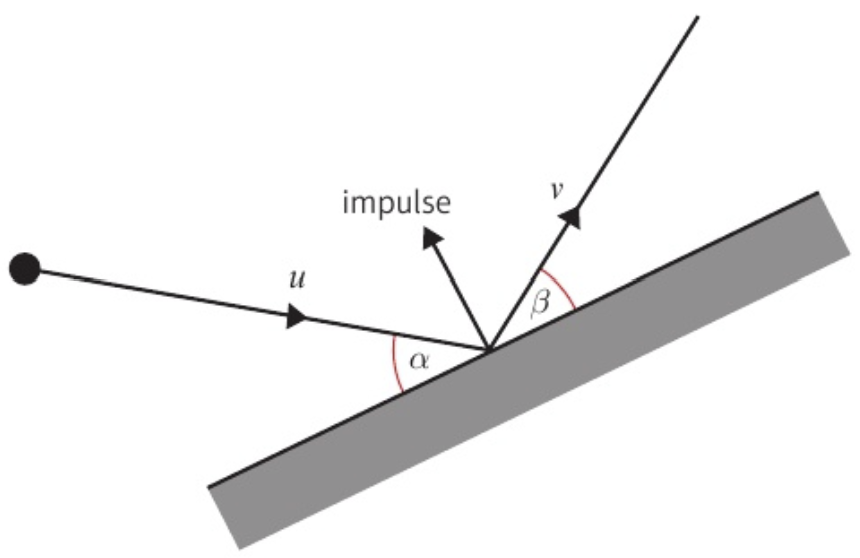
\includegraphics[width=0.3\textwidth]{obliqueimpact}
\begin{itemize}
    \item The component of the velocity of the sphere parallel to the surface is unchanged: $v\cos\beta = u\cos\alpha$
    \item The component of the velocity of the sphere perpendicular to the surface can be found with Newton's law of restitution: $v\sin\beta = eu\sin\alpha$
    \item Hence $\tan\beta = e\tan\alpha$, since $0 \leq e \leq 1$, $\beta \leq \alpha$
    \item $\text{Loss of kinetic energy}=\frac{1}{2}mu^2-\frac{1}{2}mv^2$
\end{itemize}
\section{Oblique impact of smooth spheres}
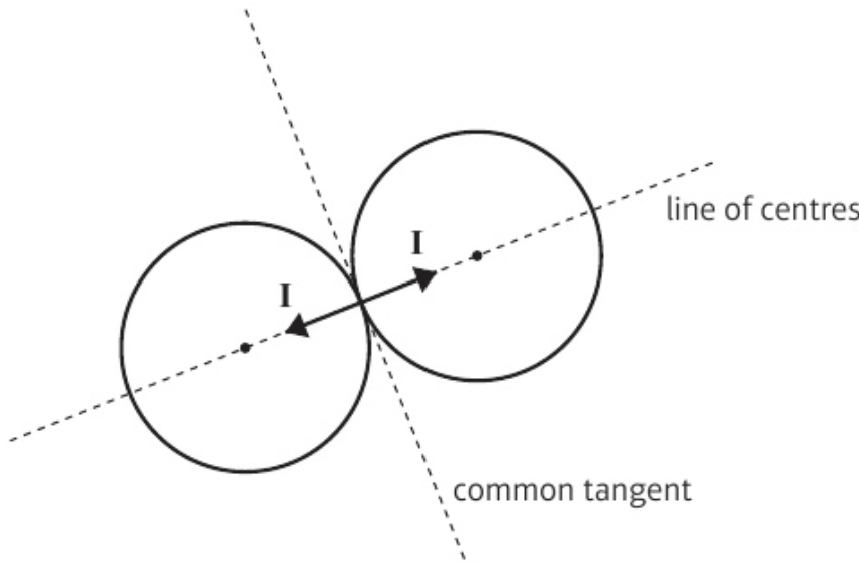
\includegraphics[width=0.3\textwidth]{oblique_2_balls}
\begin{itemize}
    \item Impulse affecting each sphere acts along the line of centres
    \item The components of the velocities of the spheres \textbf{perpendicular}  to the line of centres are unchanged in the impact
    \item The principle of conservation of momentum and Newton's law of restitution applies \textbf{parallel} to the line of centres
\end{itemize}
\chapter{Taylor series}
\section{Basic calculations}
\subsection{Addition / subtraction}
$(\mathbf {A}+\mathbf {B})_{i,j}=\mathbf {A}_{i,j}+{\mathbf {B}}_{i,j},\quad 1\leq i\leq m,\quad 1\leq j\leq n$\\
$(\mathbf {A}-\mathbf {B})_{i,j}=\mathbf {A}_{i,j}-{\mathbf {B}}_{i,j},\quad 1\leq i\leq m,\quad 1\leq j\leq n$
\subsection{Scalar multiplication}
$(c\mathbf{A})_{i,j}=c\cdot A_{i,j}$
\subsection{Matrix multiplication}
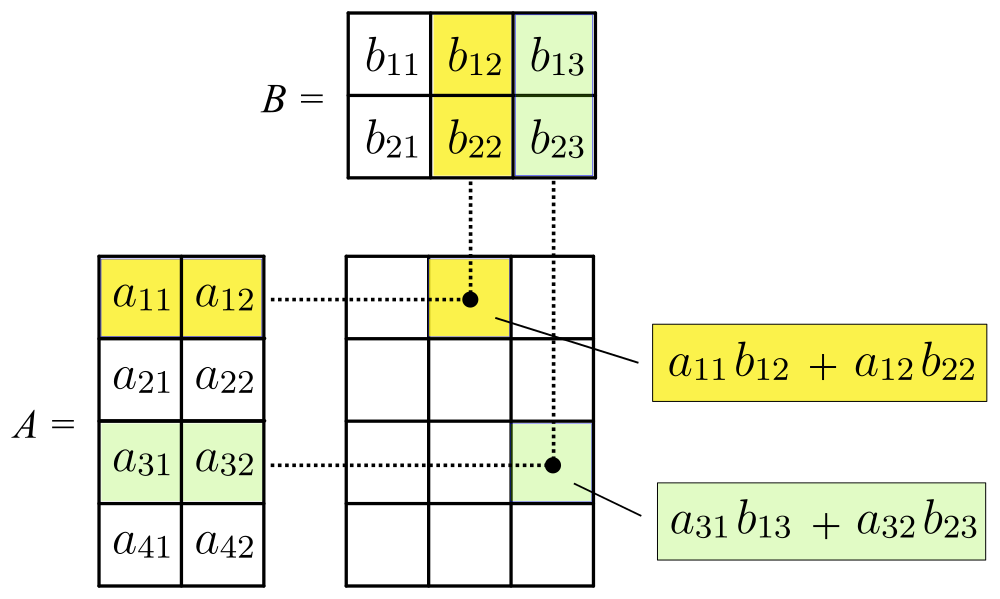
\includegraphics[width=0.35\textwidth]{MatrixMultiplication}

\subsection{Transposition}
$(\mathbf{A}^\mathrm{T})_{i,j}=A_{j,i}$

\section{Special matrices}
\begin{description}
	\item[Square matrix:] The number of rows and columns are the same
	\item[Zero matrix:] All of the elements are zero
	\item[Identity matrix:] A square matrix in which all the elements on the leading diagonal are 1 and the remaining elements are 0, denoted by $\mathbf{I}_k$ for $k\times k$ identity matrix
\end{description}


\section{Determinants}

\subsection{$2\times2$ matrices}
$\begin{vmatrix}a&b\\c&d\end{vmatrix}=ad-bc$

\subsection{$3\times3$ matrices}

$\begin{vmatrix}a&b&c\\d&e&f\\g&h&i\end{vmatrix}=a\begin{vmatrix}e&f\\h&i\end{vmatrix}-b\begin{vmatrix}d&f\\g&i\end{vmatrix}+c\begin{vmatrix}d&e\\g&h\end{vmatrix}=aei+bfg+cdh-ceg-bdi-afh$

\subsection{Singular matrices}
\begin{itemize}
	\item Singular matrices are square matrices with a determinant of 0
	\item It does not have an inverse
	\item If $\mathbf{A}$ and $\mathbf{B}$ are non-singular matrices, then $(\mathbf{AB})^{-1}=\mathbf{B}^{-1}\mathbf{A}^{-1}$
\end{itemize}



\subsection{Properties of determinants}
\begin{itemize}
	\item $\det(\mathbf{AB})=\det(\mathbf{A})\det(\mathbf{B})=\det(\mathbf{B})\det(\mathbf{A})=\det(\mathbf{BA})$
	\item $\det(k\mathbf{A})=k^n\det(\mathbf{A})$ ($\mathbf{A}$ is a $n\times n$ matrix)
\end{itemize}


\section{Inverse matrices}
\subsection{$2\times2$ matrices}
$\begin{bmatrix}
	a & b\\c & d
\end{bmatrix}^{-1}=\dfrac{1}{ad-bc}\begin{bmatrix}
	d & -b\\-c & a
\end{bmatrix}$

\subsection{$3\times3$ matrices}
$\mathbf {A} ^{-1}={\begin{bmatrix}a&b&c\\d&e&f\\g&h&i\\\end{bmatrix}}^{-1}={\frac {1}{\det(\mathbf {A} )}}{\begin{bmatrix}\,A&\,B&\,C\\\,D&\,E&\,F\\\,G&\,H&\,I\\\end{bmatrix}}^{\mathrm {T} }={\frac {1}{\det(\mathbf {A} )}}{\begin{bmatrix}\,A&\,D&\,G\\\,B&\,E&\,H\\\,C&\,F&\,I\\\end{bmatrix}}$\\
$\begin{alignedat}{6}A&={}&(ei-fh),&\quad &D&={}&-(bi-ch),&\quad &G&={}&(bf-ce),\\B&={}&-(di-fg),&\quad &E&={}&(ai-cg),&\quad &H&={}&-(af-cd),\\C&={}&(dh-eg),&\quad &F&={}&-(ah-bg),&\quad &I&={}&(ae-bd).\\\end{alignedat}$

\subsection{Solving equations with matrices}
If $\mathbf{A}\begin{pmatrix}
	x\\y\\z
\end{pmatrix}=\mathbf{v}$ then $\begin{pmatrix}
	x\\y\\z
\end{pmatrix}=\mathbf{A}^{-1}\mathbf{v}$
\begin{description}
	\item[Consistent system of linear equations:] there is at least one set of values that satisfies all the equations simultaneously
	\item[Inconsistent:] such set of values does not exist
\end{description}

\subsection{Possible outcomes of solutions}
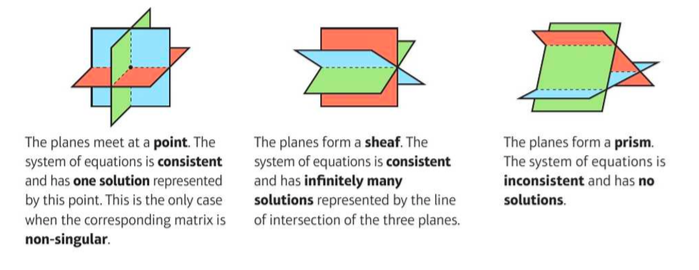
\includegraphics[width=0.75\textwidth]{equations}\\
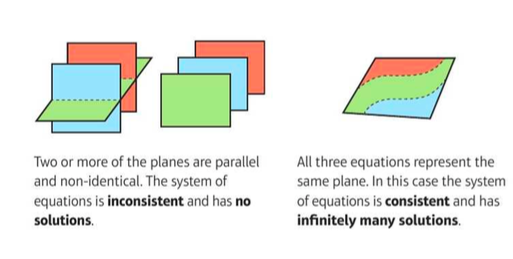
\includegraphics[width=0.5\textwidth]{equations2}
\chapter{Methods in calculus}
\section{Linear transformations in 2D}
\subsection{Properties}
If $L(\vec{v})$ is linear:
\begin{enumerate}
	\item $L(\vec{v})$ should always map the origin onto itself
	\item $L(\vec{v})$ can be represented by a matrix
	\item $L(\vec{v_1}+\vec{v_2})=L(\vec{v_1})+L(\vec{v_2})$ (closure in addition)
	\item $L(\lambda\vec{v_1})=\lambda L(\vec{v_1})$ (closure in scalar multiplication)
\end{enumerate}
\subsection{Invariant points and lines}
\begin{description}
	\item[Invariant points:] Points which are mapped onto themselves under the given transformation
	\item[Invariant lines:] Lines which map onto themselves
\end{description}

\subsection{Reflection}
\begin{description}
	\item[Reflection in $y$-axis:] $\begin{pmatrix}
		-1&0\\0&1
	\end{pmatrix}$, invariant points: points on the $y$-axis; invariant lines: $x=0$, $y=k$
	\item[Reflection in $x$-axis:] $\begin{pmatrix}
		1&0\\0&-1
	\end{pmatrix}$, invariant points: points on the $x$-axis; invariant lines: $y=0$, $x=k$
	\item[Reflection in line $y=x$:] $\begin{pmatrix}
		0&1\\1&0
	\end{pmatrix}$, invariant points: points on $y=x$; invariant lines: $y=x$, $y=-x+k$
	\item[Reflection in line $y=-x$:] $\begin{pmatrix}
		0&-1\\-1&0
	\end{pmatrix}$, invariant points: points on $y=-x$; invariant lines: $y=-x$, $y=x+k$
\end{description}

\subsection{Rotation}
\begin{description}
	\item[Rotation through angle $\theta$ anticlockwise about the origin] $\begin{pmatrix}
		\cos\theta&-\sin\theta\\\sin\theta&\cos\theta
	\end{pmatrix}$
	\item[Invariant points:] Only $(0,0)$
	\item[Invariant lines:] When $\theta=180\textdegree$ any line passing through the origin is an invariant line, otherwise no invariant lines
\end{description}

\subsection{Enlargement / stretches}
\begin{description}
	\item[Transformation matrix] $\begin{pmatrix}
		a & 0 \\ 0 & b
	\end{pmatrix}$ = a stretch of scale factor $a$ parallel to the $x$-axis and scale factor $b$ parallel to the $y$-axis
	\item[Invariant lines] $x$- and $y$-axes for all stretches
	\begin{itemize}
		\item Stretch parallel to the $x$-axes: any line parallel to the $x$-axes
		\item Stretch parallel to the $y$-axes: any line parallel to the $y$-axes
	\end{itemize}
	\item[Invariant points] The origin is always an invariant point
	\begin{itemize}
		\item Stretch parallel to the $x$-axes: points on the $y$-axes
		\item Stretch parallel to the $y$-axes: points on the $x$-axes
	\end{itemize}
	\item[Change in area] $\det(\mathbf{M}) = \text{area scale factor}$
\end{description}

\section{Linear transformations in 3D}
\begin{description}
	\item[Reflection in plane $x=0$] $\begin{pmatrix}
		-1 & 0 & 0\\
		0 & 1 & 0 \\
		0 & 0 & 1
	\end{pmatrix}$
	\item[Reflection in plane $y=0$] $\begin{pmatrix}
		1 & 0 & 0\\
		0 & -1 & 0 \\
		0 & 0 & 1
	\end{pmatrix}$
	\item[Reflection in plane $z=0$] $\begin{pmatrix}
		1 & 0 & 0\\
		0 & 1 & 0 \\
		0 & 0 & -1
	\end{pmatrix}$
	\item[Rotation angle $\theta$ anticlockwise about the $x$-axis] $\begin{pmatrix}
		1 & 0 & 0\\
		0 & \cos\theta & -\sin\theta \\
		0 & \sin\theta & \cos\theta
	\end{pmatrix}$
	\item[Rotation angle $\theta$ anticlockwise about the $y$-axis] $\begin{pmatrix}
	\cos\theta & 0 & \sin\theta \\
	0 & 1 & 0\\
	-\sin\theta & 0 & \cos\theta
	\end{pmatrix}$
	\item[Rotation angle $\theta$ anticlockwise about the $z$-axis] $\begin{pmatrix}
		\cos\theta & -\sin\theta & 0\\
		\sin\theta & \cos\theta & 0\\
		0 & 0 & 1
	\end{pmatrix}$
\end{description}





\chapter{Numerical methods}
\section{Hyperbolic function definitions}
\subsection{$\sinh x$}
\begin{description}
	\item[Definition] $\sinh x = \dfrac{e^x-e^{-x}}{2}$
	\item[Domain] $x \in \textbf{R}$
	\item[Asymptotes] $x\rightarrow +\infty$, $y\rightarrow\dfrac{e^x}{2}$; $x\rightarrow -\infty$, $y\rightarrow -\dfrac{e^{-x}}{2}$
	\item[x-intercept] $(0,0)$
	\item[y-intercept] $(0,0)$
	\item[Graph]
\end{description}

\subsection{$\cosh x$}
\begin{description}
	\item[Definition] $\cosh x = \dfrac{e^x+e^{-x}}{2}$
	\item[Domain] $x \in \textbf{R}$
	\item[Asymptotes] $x\rightarrow +\infty$, $y\rightarrow\dfrac{e^x}{2}$; $x\rightarrow -\infty$, $y\rightarrow\dfrac{e^{-x}}{2}$
	\item[x-intercept] No
	\item[y-intercept] $(0,1)$
	\item[Graph]
\end{description}

\subsection{$\tanh x$}
\begin{description}
	\item[Definition] $\tanh x = \dfrac{\sinh x}{\cosh x}=\dfrac{e^x-e^{-x}}{e^x+e^{-x}}$
	\item[Domain] $x \in \textbf{R}$
	\item[Asymptotes] $x\rightarrow +\infty$, $y\rightarrow 1$; $x\rightarrow -\infty$, $y\rightarrow -1$
	\item[x-intercept] $(0,0)$
	\item[y-intercept] $(0,0)$
	\item[Graph]
\end{description}

\subsection{$\csch x$}
\begin{description}
	\item[Definition] $\csch x = \dfrac{1}{\sinh x}$
	\item[Domain] 
	\item[Asymptotes] 
	\item[x-intercept] 
	\item[y-intercept] 
	\item[Graph]
\end{description}


\subsection{$\sech x$}
\begin{description}
	\item[Definition] $\sech x = \dfrac{1}{\cosh x}$
	\item[Domain] 
	\item[Asymptotes] 
	\item[x-intercept] 
	\item[y-intercept] 
	\item[Graph]
\end{description}


\subsection{$\coth x$}
\begin{description}
	\item[Definition] $\coth x = \dfrac{\cosh x}{\sinh x}$
	\item[Domain] 
	\item[Asymptotes] 
	\item[x-intercept] 
	\item[y-intercept] 
	\item[Graph]
\end{description}

\section{Identities of hyperbolic functions}
Similar to trigonometric identities:
\begin{itemize}
	\item $\tanh x = \dfrac{\sinh x}{\cosh x}$
	\item $\cosh^2 x - \sinh^2 x = 1$
	\item $\tanh^2 x + \sech^2 x= 1$
	\item $\coth^2 x - \csch^2 x = 1$
\end{itemize}

\subsection{Addition}
\begin{itemize}
	\item $\sinh(x+y)=\sinh x \cosh y + \sinh y \cosh x$
	\item $\cosh(x+y)=\cosh x \cosh y + \sinh x \sinh y$
	\item $\tanh(x+y) = \dfrac{\sinh(x+y)}{\cosh(x+y)} = \dfrac{\sinh x \cosh y + \sinh y \cosh x}{\cosh x \cosh y + \sinh x \sinh y} = \dfrac{\frac{\sinh x}{\cosh x}+\frac{\sinh y}{\cosh y}}{1 + \frac{\sinh x \sinh y}{\cosh x \cosh y}}=\dfrac{\tanh x + \tanh y}{1 + \tanh x \tanh y}$
\end{itemize}

\subsection{Double angle}
\begin{itemize}
	\item $\sinh 2x = 2\sinh x \cosh x$
	\item $\cosh 2x = \cosh^2 x + \sinh^2 x = 2\cosh^2 x - 1 = 2\sinh^2 + 1$
	\item $\tanh 2x = \dfrac{2\tanh x}{1 + \tanh^2 x}$
\end{itemize}

\subsection{Power descending}


\section{Differentiating hyperbolic functions}
\begin{itemize}
	\item $(\sinh x)'=\cosh x$
	\item $(\cosh x)'=\sinh x$
	\item $(\tanh x)'=1-\tanh^2 x = \sech^2 x$
	\item $(\csch x)'=-\coth x \csch x$
	\item $(\sech x)'=-\sech x \tanh x$
	\item $(\coth x)'=-\sech^2 x$
\end{itemize}
\chapter{Redicible differential equations}
\section{SUVAT equations}
\begin{itemize}
    \item $s=ut+\dfrac{1}{2}at^2$
    \item $s=vt-\dfrac{1}{2}at^2$
    \item $v=u+at$
    \item $v^2=u^2+2as$
    \item $s=\dfrac{1}{2}(u+v)t$
\end{itemize}



\end{document}